\chapter{Introduction}
\label{Introduction}
{This is an overview of the main techniques of media streaming in the past years. It interpretes the phylogeny of media content delivery system, which includes from the traditional client-server framework to the Peer-to-Peer mesh network topology based delivery method system. And also, it will contain the main extra knowledge about P2P system and video media encapsulation techniques, which was widely used in current media player codec software , such as Gstreaming, VLC, and many other open source softwares.}

\section{Traditional C/S Architecture based Streaming}
{
  Traditional C/S Architecture based media content delivery system, which once occupied a high rate market share in old days, has its advantages in many points. Because of its centralised resources management and server level administration, many applications were designed and implemented in this kind of network environment. Thanks to this architecture it is possible to remove or add clients without affecting the operation of the network and without the need for major modification.

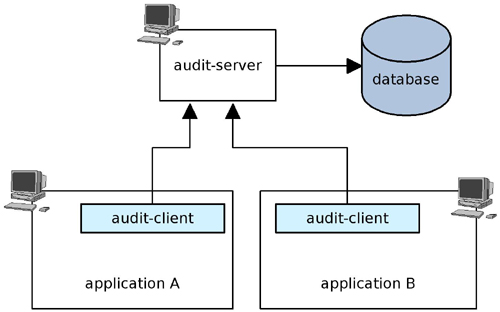
\includegraphics[width=10cm]{data/architecture-small.jpg}
\\

However, due to the technical complexity of the server, the sever will be the only weakness in this architecture. The large number of clients access the same server, which will lead to traffic congestion, that directly affects the performance and fault-tolerance requirment of video delivery system.

In traditional C/S model, all of the media data interchangement should involve server machine, as the growth of client quantity, server will become the bottleneck of whole video delivery system. Once the Server crashed, and the whole system will crashed as well. Secondly, C/S based video delivery system totally depends on the central node -- server. It can not work without server node, and then it will be meaningless of the whole network. Thirdly, there are a great volume of idle resources in client end (such as disk usage, CPU circle). If the client dose not get the response from server, all of the resurce will be dissipated. This will absolutely lead to a low resource utilization.
}

\subsection{RTP/RTSP protocol based live Video Streaming}
{
RTP is a transport protocol for the delivery of real-time data, including interactive streaming audio and video under single broadcast or group multicast environment. 
Applications usually run RTP based on UDP protocol, in order to mux the usage of multi-node and inspection services;even both of the two protocols contain the transport layer protocol functions.
However, RTP can be integrated with the other suiteable underlying netork or transport protocol. 
If the underlying network support group multicast service , RTP can use the multicast table to deliver the data to multiple destinations.

RTP does not support delivering on time mechanism or any other \emph{QOS} assurance. That means RTP can not ensure avoiding disorderly transfer or the reliability of the underlying network. However, RTP is a orderly transfer protocol. The Serial Number in RTP transfer session enabled the recipient to restruct the serial packages.

RTCP is a part of RTP and helps with lip synchronization and QOS management, among others, which also can provide the infomation about transfer members in the session. The second aspection of RTCP functions is enough for \emph{Loosely controlled} session, that means, if there is no specific memeber to control or orgnize, it does not have to be used as an application which can control all of the communicate requests.

\begin{center}
\begin{tabular}{@{}llllll@{}}\toprule
1   & 2 &   3 &   8             &           9      & 16bit\\\midrule
V 	& P &   X &   CSRC Count 	&           M 	   &Payload Type\\
\multicolumn{4}{c} {Sequence number}               &  Timestamp\\
\multicolumn{4}{c}{SSRC} 	    &\multicolumn{2}{{c}}{CSRC (variable 0 – 15 items 32bits each)}\\
\bottomrule
\end{tabular}
\end{center}
\footnote{The table indicates RTP package elements, more detail information can be refered in RTP wiki page \url{http://en.wikipedia.org/wiki/Real-time_Transport_Protocol}}
\begin{itemize}
\item V -- Version,indicates the version of the protocol.
\item P -- Padding,used to indicate if there are extra padding bytes at the end of the RTP packet.
\item X -- Extension,indicates presence of an Extension header between standard header and payload data.x
\item CC --Contains the number of CSRC identifiers (defined below) that follow the fixed header.
\item M -- Marker,Used at the application level and defined by a profile.
\item PT -- Indicates the format of the payload and determines its interpretation by the application. 
\item SN -- Sequence number,incremented by one for each RTP data packet sent and is to be used by the receiver to detect packet loss and to restore packet sequence.
\item TT -- Timestamp ,Used to enable the receiver to play back the received samples at appropriate intervals.
\item SSRC -- Synchronization source identifier uniquely identifies the source of a stream. 
\item CSRC -- Contributing source IDs enumerate contributing sources to a stream which has been generated from multiple sources.
\end{itemize}

RTSP is a control protocol that initiating and directing delivery of streaming multimedia from media servers, the "Internet VCR remote control protocol". 
RTSP does not deliver data (though the RTSP connection may be used to tunnel RTP traffic for ease of use with firewalls and other network devices). 
The proposed standard of RTSP has been defined in RFC2326, which was widely used in media stream transmission. At present, most of the resolvents on real and quick time media stream are support RTSP protocol.

The design and implement of RTSP is similar to HTTP protocol. The relationship between RTSP and RTP/RTCP is familar with the one between HTTP and TCP. But still, there is much diversity. RTSP is a durable link in the process of media stream dibbling and palyback. So, no matter Client or Server can have a state. However, there is no state in HTTP protocol; HTTP status information needs other ancillary mechanism to maintain,such as \emph{Cookie}. In addition, RTSP does not use the RTP / RTCP, but to manipulate them, and itself is still using the TCP protocol. The HTTP uses TCP transport.
Demand that the entire media and playback process is a Session, Session embodies a state machine, Client and Server have a state machine each.

The state machine of client are as followed, and the events are receiveed from user input.
\begin{center}
\begin{tabular}{@{}lll@{}}\toprule
                    &       EVENT                &    TARGET \\ \midrule
                    &       TEARDOWN             &     Init\\  
   Init             &       SETUP                &      Ready \\ \midrule
   Ready            &       PLAY                 &      Playing \\
                    &       RECORD               &     Recording\\
                    &       TEARDOWN             &      Init\\
                    &       SETUP                &      Ready\\\midrule
   Playing          &      PAUSE                 &      Ready\\ 
                    &     TEARDOWN               &      Init\\
                    &      PLAY                  &      Playing\\
                    &     SETUP                  &      Playing \\\midrule
   Recording        &      PAUSE                 &      Ready\\ 
                    &     TEARDOWN               &      Init\\
                    &     RECORD                 &      Recording\\
                    &      SETUP                 &      Recording \\\bottomrule
\end{tabular}
\end{center}
The Serve state machine also contains the four states, state transition rules are the same, but the object and the semantic differential.
As reference HTTP, The text format of RTSP protocol is similar to the HTTP's, accurate to say that should be used in rfc822. every line of text separated by a CRLF.

}
\subsection{MMS Protocol based Video Streaming}
{

Microsoft Media Server (MMS) is the name of Microsoft's proprietary network streaming protocol used to transfer unicast data in Windows Media Services (previously called NetShow Services).\footnote{\url{http://en.wikipedia.org/wiki/Microsoft_Media_Server}}
If the audience in Windows Media Player to connect to the typed URL, rather than through a hyperlink to access the content, they must use the MMS protocol to reference the stream. When using the MMS protocol to connect to the distribution point, you can use 'protocol rollover' to get the best connection. While trying to use MMSU to connect the client point,"Protocol rollover" begins to take over the original connection. MMST is the combination of MMS protocol UDP data transfer. If MMSU connection is not successful, the server will attempt to use MMST. 
MMST is the MMS protocol with TCP data transfer.

If connected to the indexed Asf file, and you want to do fast forward, rewind, pause, start and stop the stream, you must use MMS. That was because UNC paths can not do fast forward or backward.
When connecting to the distrituted points with independent Windows Media Player, you have to specify the unicast content of URL. 
}


\section{P2P Architecture based Streaming}
{
  As the development of the information network, the demand of stream media is growing.  However, most traditional stream media service uses C/S mode,which connects to each client with unicast method. Because streaming media service is with high bandwidth and long duration, as the number of clients growing, the resource of server will be consumed very soon, which then becomes the bottleneck of whole system. As to these problems, the main solution recently is to use content dilivery network (\emph{CDN}) , and IP muiltcast. The main tech of CDN is to use proxy server which can copy the media data ,and deliver them to multiple destinations. However, this tech requres high cost, which still be the most important defect to deploy CDN in the global. As to IP multicast,because of the limitations of its own (such as hardly implementation of QOS of multicast,control of congestion, and complexity of the protocol), IP multicast is not wildely used. P2P overlay network  brings a new solution to media streaming. In the Peer to Peer network, each peer entity takes role of both server and client , which distributes the load of server to each peer. So it balances the load of the server and reduces the usage of network bandwidth ,which improved scalability of the whole system.
}

\subsection{Framework of P2P media streaming}
{
According to the way of source node delivering data, P2P media streaming system can be categorized as two types: single-source P2P media streaming transmission and multi-sources media streaming transmission. 

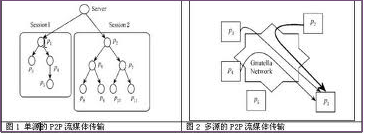
\includegraphics[width=8cm]{data/P2Pframework.png}

Single-source P2P media streaming transmission is based on application layer multicast tech, which is a tree-based multi-layer structure. 
There is a single source sender and multipule data receivers, and each receiver acquires data only from one sender. The server and all of the peer nodes make up of a multicast tree structure. 
The node of the multicast tree receives data from its father node, and then deliver the data to its child-nodes with multicast method. 
In this structure, each client machine only acquires data from the up level nodes, so the up level nodes affect the performance of the whole system more directly. 
However, the users in the internet can not assure the quality of service, so it will be hard to maintain a stable tree-based structure. 
More over, due to the limitation of the client machines, the growth of new users which directly leads to the increasing level of the tree structure, will bring up the delayer time of the leaf machines. And the leaf nodes does not service the up level machines, so the  system can not take full advantage of the network resources.

The structure of multi-sources media streaming system is netted texture. Multipule senders transmit the data to the same receiver. Each client acquries data from multipule clients or servers segregatedly. 
The data in the buffer is divided into chunks that is with the same size. And the client sends data requests to multipule clients to acquire specify data chunk, according to a certain policy. 
In this way, the speed of data delivery can be promoted in a short time. However , this technique is complex , which involve the way to chosse sender peer, coordinate the transfer rate of multipule sender peers, and the way to allocate data segment on specific sender peers.
}

\subsection{Techniques of P2P media Streaming delivering}
{
 At present, there are two types of P2P media streaming delivering techniques:
\begin{enumerate}
\setcounter{enumi}{0}
\item Tree-based protocol and extensions. In this mode, the nodes will be organised as a multicast tree. The parent node in the tree will take responsibility for delivering media data. More attention will focus on the construction and balance of the multicast tree.
\item Gossip-based protocol. Gossip algorithm is the most popular in P2P system for delivering message. In a typical \emph{Gossip} algorithm, node will send messages to some of the nodes according to a random list, and the nodes received data will deliver the messages to the other nodes. Repeat this process , until the message has been received by all of the nodes in this P2P system. 
The media streaming system based on \emph{Gossip} algorithm does not construct the topology between nodes exhibitly, but maintain the view between each node and the some of the other nodes though the \emph{Gossip} algorithm. 
Each node will exchange the cached infomation with the other nodes, and exchange the media data according the cached infomation. In this kind of system, more buffer and more waiting time for system setting up will be required.
\end{enumerate}
}

\section{OGG Vobis bitstream encapsulation}
{
  The \emph{OGG bitstream} format has been developed as a part of a larger project aimed at creating a set of components for the coding and decoding of multimedia content (codecs) which are to be freely avaliable and free re-implementable, both in software and in hardware for the computing community at large, including the Internet community.\cite{oggencapsulationformat}. More Glossary of terms and abbreviations, please refer to Appendix A which is a part of RFC3533.
}
\subsection{The Ogg bitstreaem format} 
{
The physical Ogg bitstream is composed by multiple logical bitstreams which is so-called "Pages".  
The logical bitstreams are identified by a unique serial number in the header of each page of the physical bitstream.  
This unique serial number is created randomly and does not have any connection to the content or encoder of the logical bitstream it represents. \cite{oggencapsulationformat}  
The data of each Ogg page is unique, beacause it belongs to specific one logical bitstream only. 
And the size of ogg pages are variable, which contains header encapuslation and error recovery infomation.
Each logical bitstream in a physical Ogg bitstream starts with a special start page (bos=beginning of stream) and ends with a special page (eos=end of stream).The bos page contains information to uniquely identify the codec type and MAY contain information to set up the decoding process. The format of the bos page is dependent on the codec and therefore MUST be given in the encapsulation specification of that logical bitstream type. \cite{oggencapsulationformat}


There are two types of multiplexing of \emph{Ogg}: Grouping and Chaining.
Grouping deines the way to interleave multipule logical bitstreams in the same physical bitstream.
Chaining on the other hand, is define to concatenate physical ogg bitstreams.
In grouping, all bos pages of all logical bitstreams should appear at the beginning of the Ogg bitstream.But all of eof pages are not required to appear at the end of this streaming.
In Chaining, there is not overlap of each bitstreams. However, the chained bitstream should contain a unique serial number within the scope of the physical bitstream.
}

\subsection{The ogg page format}
{
The Ogg page header has the following format:

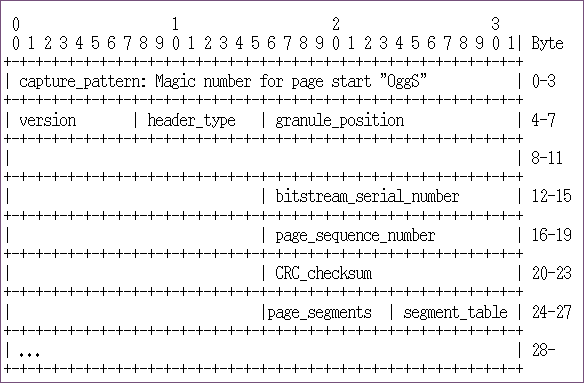
\includegraphics[width=12cm]{data/oggpageheader.png}       

\begin{itemize}
\item capture pattern -- a 4 Byte field that signifies the beginning of a
       page.  It contains the magic numbers:
             0x4f 'O'
             0x67 'g'
             0x67 'g'
             0x53 'S'
\item stream structure version -- 1 Byte signifying the version number of the Ogg file format used in this stream
\item header type flag -- the bits in this 1 Byte field identify the specific type of this page.
\item granule position -- an 8 Byte field containing position information.
\item bitstream serial number -- a 4 Byte field containing the unique
       serial number by which the logical bitstream is identified.
\item page sequence number -- a 4 Byte field containing the sequence
       number of the page so the decoder can identify page loss.  This
       sequence number is increasing on each logical bitstream
       separately.
\item CRC checksum -- a 4 Byte field containing a 32 bit CRC checksum of
       the page (including header with zero CRC field and page content).
       The generator polynomial is 0x04c11db7.
\item number page segments -- 1 Byte giving the number of segment entries
       encoded in the segment table.
\item segment table -- number page segments Bytes containing the lacing
       values of all segments in this page.  Each Byte contains one
       lacing value.
\end{itemize}
%   The total header size in bytes is given by:
%    header_size = number_page_segments + 27 [Byte]\\
%    The total page size in Bytes is given by:
%   page_size = header_size + sum(lacing_values: 1..number_page_segments)[Byte]
}
\section{Contributions}
{
  The Contributions of this thesis are as follow:
\begin{itemize}
\item I study the current P2P network on VoD solutions and their design decisions. Especially I anaylse the coedc and containers that enables kadpeer VoD functions to be implemented.
\item I modified the codec moudule of the Oggplayer to manage meta data and stream data effectively , and used SDL librarys to do stream rollback playing.
\item I illustrate a effective method of media files splitting and publishing which allows users to get the updated resources more easily.
\item Much efforts have been paied on the implementation of \emph{Kademlia} Algorithm which is the only P2P network we analyse and module in this thesis. Many other common modules are involved in kadpeer design and implementation.
\end{itemize}
}
\section{Summary}
{
In this chapter, I have illustrated the core architectures that are used widely in media stream infrastructure, and the common techniques of each mode. 
RTP/RTSP and MMS protocols have been supported steadily in many kinds of media player or other stream applications,and much many open source groups have implemented these protocols. 
The two frameworks of P2P are sinlge-source and multi-sources transmission. And the main alogrithm of data delivering are Tree-based protocol and extension and Gossip demagogy.
Moreover, in the last section, i present the basic knowledge about the Ogg encapsulation of media stream, which has been as a low-layer method to deliver bitstream in \emph{kadpeer} project. And I used open source \emph{liboggz} as a third part library which is with GPL2 license for modifing and contribution.
}
